\documentclass{beamer}
\usetheme[block = fill, titleformat title = allcaps, titleformat subtitle  = smallcaps,
progressbar = foot, background = light]{metropolis}           % Use metropolis theme
\usepackage{pgfplots}
\usetikzlibrary{arrows.meta,positioning, shapes, backgrounds}
\title{Housing market and migration revisited}
\subtitle{A Bayesian multilevel gravity model for Dutch municipalities}
\date{\today}
\author{Thomas de Graaff}
\institute{Vrije Universiteit Amsterdam\\Department of Spatial Economics}
\begin{document}
\maketitle

\begin{frame}{Background: two different cultures (following Breiman, 2001)}
	\begin{columns}
		\begin{column}{0.5\textwidth}
			In economics: 
			\begin{itemize}
				\item \textbf{causal }impact of $x$ on $y$
				\item \textbf{Average} treatment effect
		    \end{itemize}
			\begin{center}
				\includegraphics[width=0.5\textwidth]{../fig/harmless}      
			\end{center}
		\end{column}\pause
		\begin{column}{0.5\textwidth} 
		Outside economics: 
			\begin{itemize}
				\item \textbf{Model performance } 
				\item \textbf{prediction} of total effect
			\end{itemize}
			\begin{center}
				\includegraphics[width=0.5\textwidth]{../fig/rethinking}      
			\end{center}
		\end{column}
	\end{columns}
\end{frame}

  \begin{frame}{Background}
    	\begin{itemize}
    		\item 50--70\% of all research questions in spatial economics evolve around policy \alert{evaluation} 
    		\begin{itemize}
    			\item focus on \textbf{consistency}
    		\end{itemize}
    		\item Huge demand (e.g., by firms \& government) for research dealing with \alert{prediction}
    		\begin{itemize}
    			\item focus on model \textbf{performance}
    		\end{itemize}
    		\item But, more than 90\% of all statistical analyses is basic applied econometrics using \alert{linear} models and \alert{fixed} effects
    	\end{itemize}
  \end{frame}

\begin{frame}{Research question}
	\begin{itemize}
		\item Aggregate homeownership has negative impact on labour market performance, because of increased \alert{moving costs} (Oswald, 1996, 1999)
		\item This paper applies a \alert{gravity model} on the impact of housing market structure (e.g., homeownership and social renting) on within-country migration flows (Congdon, 2010)
		\item \textbf{Aim}: to be able to \alert{predict} all changes in incoming and outcoming migration flows of, e.g., Amsterdam, when housing market structure changes \alert{whilst} accounting for origin and destination specific effects (Ranjan \& Tobias, 2007)
	\end{itemize}
\end{frame}

\begin{frame}[fragile]{Gravity model data structure}
	 \begin{figure}	
   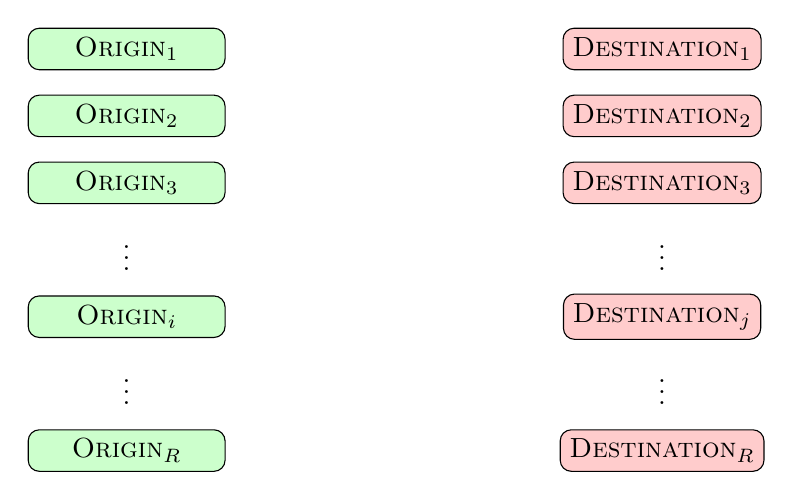
\begin{tikzpicture}[scale=0.85, thick]
   
   \tikzstyle{orig}=[rectangle, rounded corners, thin, fill=green!20, text=black, draw, minimum width=2.5cm]
   \tikzstyle{dest}=[rectangle, rounded corners, thin, fill=red!20, text=black, draw, minimum width=2.5cm]
   \tikzstyle{migrants}=[rectangle, rounded corners, thin, fill=blue!20, text=black, draw, minimum width=2.5cm]
   \tikzstyle{var}=[rectangle, rounded corners, thin, fill=black!10, text=black, draw, text width = 3.5cm]
   
   \node[orig] (o1) at (0,0)  {\textsc{Origin$_1$}};
   \node[orig] (o2) at (0,-1) {\textsc{Origin$_2$}};
   \node[orig] (o3) at (0,-2) {\textsc{Origin$_3$}};
   \node (o4) at (0,-3) {\textsc{\vdots}};
   \node[orig] (o5) at (0,-4) {\textsc{Origin$_i$}};
   \node (o6) at (0,-5) {\textsc{\vdots}};
   \node[orig] (o7) at (0,-6) {\textsc{Origin$_R$}};
   
   \node[dest] (d1) at (8,0)  {\textsc{Destination$_1$}};
   \node[dest] (d2) at (8,-1) {\textsc{Destination$_2$}};
   \node[dest] (d3) at (8,-2) {\textsc{Destination$_3$}};
   \node (d4) 		 at (8,-3) {\textsc{\vdots}};
   \node[dest] (d5) at (8,-4) {\textsc{Destination$_j$}};
   \node (d6) 		 at (8,-5) {\textsc{\vdots}};
   \node[dest] (d7) at (8,-6) {\textsc{Destination$_R$}};
%   
%   % Migratior links
%   \draw[-latex, blue, thin, dashed] (1.5,0) -- (6.5, 0);
%   \draw[-latex, blue, thin, dashed] (1.5,0) -- (6.5,-0.8);
%   \draw[-latex, blue, thin, dashed] (1.5,0) -- (6.5,-1.8);
%   \draw[-latex, blue, thin, dashed] (1.5,0) -- (6.5,-3.8);
%   \draw[-latex, blue, thin, dashed] (1.5,0) -- (6.5,-5.6);
%   
%   \draw[-latex, blue, thin, dashed] (1.5,-1) -- (6.5,-0.1);
%   \draw[-latex, blue, thin, dashed] (1.5,-1) -- (6.5,-0.9);
%   \draw[-latex, blue, thin, dashed] (1.5,-1) -- (6.5,-1.9);
%   \draw[-latex, blue, thin, dashed] (1.5,-1) -- (6.5,-3.9);
%   \draw[-latex, blue, thin, dashed] (1.5,-1) -- (6.5,-5.7);
%   
%   \draw[-latex, blue, thin, dashed] (1.5,-2) -- (6.5, -0.2);
%   \draw[-latex, blue, thin, dashed] (1.5,-2) -- (6.5,-1);
%   \draw[-latex, blue, thin, dashed] (1.5,-2) -- (6.5,-2);
%   \draw[-latex, blue, thin, dashed] (1.5,-2) -- (6.5,-4);
%   \draw[-latex, blue, thin, dashed] (1.5,-2) -- (6.5,-5.8);
%   
%   \draw[-latex, blue, thin, dashed] (1.5,-4) -- (6.5,-0.3);
%   \draw[-latex, blue, thin, dashed] (1.5,-4) -- (6.5,-1.1);
%   \draw[-latex, blue, thin, dashed] (1.5,-4) -- (6.5,-2.1);
%   \draw[-latex, blue, thin, dashed] (1.5,-4) -- (6.5,-4.1);
%   \draw[-latex, blue, thin, dashed] (1.5,-4) -- (6.5,-5.9);
%   
%   \draw[-latex, blue, thin, dashed] (1.5,-6) -- (6.5, -0.4);
%   \draw[-latex, blue, thin, dashed] (1.5,-6) -- (6.5,-1.2);
%   \draw[-latex, blue, thin, dashed] (1.5,-6) -- (6.5,-2.2);
%   \draw[-latex, blue, thin, dashed] (1.5,-6) -- (6.5,-4.2);
%   \draw[-latex, blue, thin, dashed] (1.5,-6) -- (6.5,-6);
%   
%   \node[migrants] (m) at (4,-3)  {\textsc{Migrant flows $i \rightarrow j$}};
%   
%   \node[var] (v1) at (0,-8)  {\textsc{Origin-specific variables ($o_i, \mathbf{X_i}$)}};
%   \node[var] (v2) at (4,-8)  {\textsc{flow-specific variables ($\mathbf{X}_{ij}$) }};
%   \node[var] (v3) at (8,-8)  {\textsc{Destination-specific variables  ($d_j, \mathbf{X_j}$)}};
%   
%   \begin{pgfonlayer}{background}
%   \filldraw [line width=4mm,join=round,black!10]
%   (o1.north -| o1.west)  rectangle (o7.south -| o7.east)
%   (d1.north -| d1.west)  rectangle (d7.south -| d7.east);
%   \end{pgfonlayer}
%   
%   \draw[-latex, thick, black] (v1) -- (0,-6.5);
%   \draw[-latex, thick, black] (v2) -- (4,-6.5);
%   \draw[-latex, thick, black] (v3) -- (8,-6.5);
   \end{tikzpicture}
	\end{figure}
\end{frame}

\begin{frame}[fragile]{Gravity model data structure}
	\begin{figure}	
		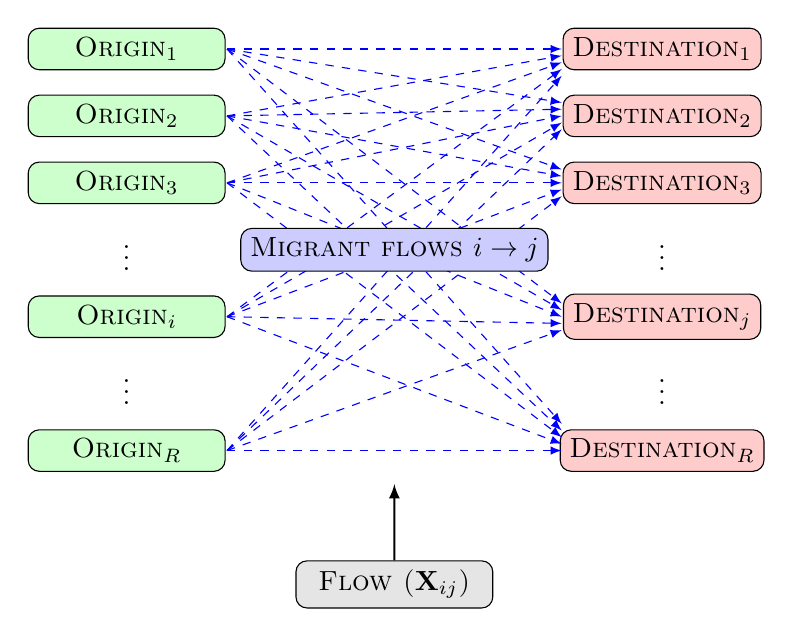
\begin{tikzpicture}[scale=0.85, thick]
		
		\tikzstyle{orig}=[rectangle, rounded corners, thin, fill=green!20, text=black, draw, minimum width=2.5cm]
		\tikzstyle{dest}=[rectangle, rounded corners, thin, fill=red!20, text=black, draw, minimum width=2.5cm]
		\tikzstyle{migrants}=[rectangle, rounded corners, thin, fill=blue!20, text=black, draw, minimum width=2.5cm]
		\tikzstyle{var}=[rectangle, rounded corners, thin, fill=black!10, text=black, draw, minimum width = 2.5cm]
		
		\node[orig] (o1) at (0,0)  {\textsc{Origin$_1$}};
		\node[orig] (o2) at (0,-1) {\textsc{Origin$_2$}};
		\node[orig] (o3) at (0,-2) {\textsc{Origin$_3$}};
		\node (o4) at (0,-3) {\textsc{\vdots}};
		\node[orig] (o5) at (0,-4) {\textsc{Origin$_i$}};
		\node (o6) at (0,-5) {\textsc{\vdots}};
		\node[orig] (o7) at (0,-6) {\textsc{Origin$_R$}};
		
		\node[dest] (d1) at (8,0)  {\textsc{Destination$_1$}};
		\node[dest] (d2) at (8,-1) {\textsc{Destination$_2$}};
		\node[dest] (d3) at (8,-2) {\textsc{Destination$_3$}};
		\node (d4) 		 at (8,-3) {\textsc{\vdots}};
		\node[dest] (d5) at (8,-4) {\textsc{Destination$_j$}};
		\node (d6) 		 at (8,-5) {\textsc{\vdots}};
		\node[dest] (d7) at (8,-6) {\textsc{Destination$_R$}};
		   
		   % Migratior links
		   \draw[-latex, blue, thin, dashed] (1.5,0) -- (6.5, 0);
		   \draw[-latex, blue, thin, dashed] (1.5,0) -- (6.5,-0.8);
		   \draw[-latex, blue, thin, dashed] (1.5,0) -- (6.5,-1.8);
		   \draw[-latex, blue, thin, dashed] (1.5,0) -- (6.5,-3.8);
		   \draw[-latex, blue, thin, dashed] (1.5,0) -- (6.5,-5.6);
		   
		   \draw[-latex, blue, thin, dashed] (1.5,-1) -- (6.5,-0.1);
		   \draw[-latex, blue, thin, dashed] (1.5,-1) -- (6.5,-0.9);
		   \draw[-latex, blue, thin, dashed] (1.5,-1) -- (6.5,-1.9);
		   \draw[-latex, blue, thin, dashed] (1.5,-1) -- (6.5,-3.9);
		   \draw[-latex, blue, thin, dashed] (1.5,-1) -- (6.5,-5.7);
		   
		   \draw[-latex, blue, thin, dashed] (1.5,-2) -- (6.5, -0.2);
		   \draw[-latex, blue, thin, dashed] (1.5,-2) -- (6.5,-1);
		   \draw[-latex, blue, thin, dashed] (1.5,-2) -- (6.5,-2);
		   \draw[-latex, blue, thin, dashed] (1.5,-2) -- (6.5,-4);
		   \draw[-latex, blue, thin, dashed] (1.5,-2) -- (6.5,-5.8);
		   
		   \draw[-latex, blue, thin, dashed] (1.5,-4) -- (6.5,-0.3);
		   \draw[-latex, blue, thin, dashed] (1.5,-4) -- (6.5,-1.1);
		   \draw[-latex, blue, thin, dashed] (1.5,-4) -- (6.5,-2.1);
		   \draw[-latex, blue, thin, dashed] (1.5,-4) -- (6.5,-4.1);
		   \draw[-latex, blue, thin, dashed] (1.5,-4) -- (6.5,-5.9);
		   
		   \draw[-latex, blue, thin, dashed] (1.5,-6) -- (6.5, -0.4);
		   \draw[-latex, blue, thin, dashed] (1.5,-6) -- (6.5,-1.2);
		   \draw[-latex, blue, thin, dashed] (1.5,-6) -- (6.5,-2.2);
		   \draw[-latex, blue, thin, dashed] (1.5,-6) -- (6.5,-4.2);
		   \draw[-latex, blue, thin, dashed] (1.5,-6) -- (6.5,-6);
		   
		   \node[migrants] (m) at (4,-3)  {\textsc{Migrant flows $i \rightarrow j$}};
		   
		%   \node[var] (v1) at (0,-8)  {\textsc{Origin-specific variables ($o_i, \mathbf{X_i}$)}};
		   \node[var] (v2) at (4,-8)  {\textsc{Flow ($\mathbf{X}_{ij}$) }};
		%   \node[var] (v3) at (8,-8)  {\textsc{Destination-specific variables  ($d_j, \mathbf{X_j}$)}};
		%   
		%   \begin{pgfonlayer}{background}
		%   \filldraw [line width=4mm,join=round,black!10]
		%   (o1.north -| o1.west)  rectangle (o7.south -| o7.east)
		%   (d1.north -| d1.west)  rectangle (d7.south -| d7.east);
		%   \end{pgfonlayer}
		%   
		%   \draw[-latex, thick, black] (v1) -- (0,-6.5);
		   \draw[-latex, thick, black] (v2) -- (4,-6.5);
		%   \draw[-latex, thick, black] (v3) -- (8,-6.5);
		\end{tikzpicture}
	\end{figure}
\end{frame}

\begin{frame}[fragile]{Gravity model data structure}
	\begin{figure}	
		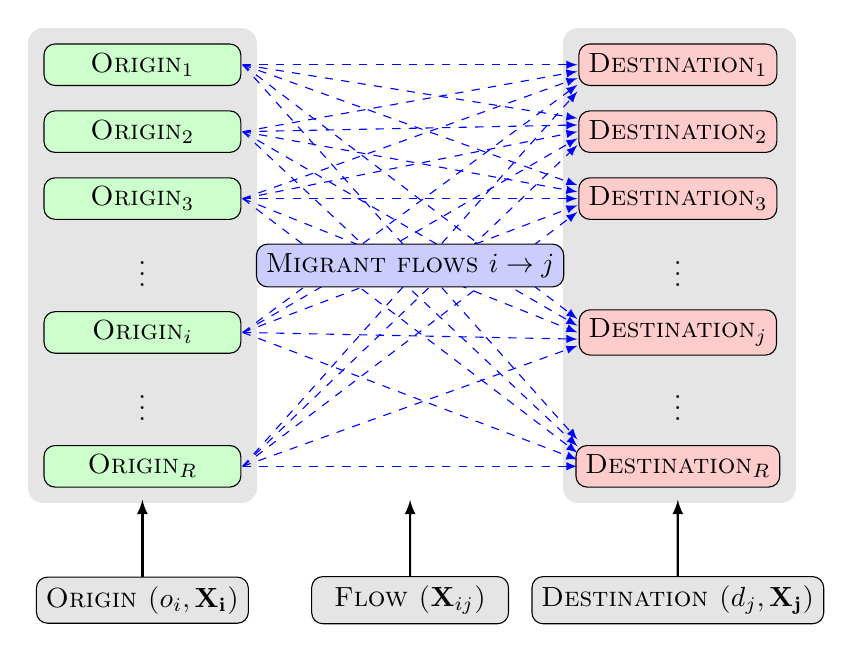
\begin{tikzpicture}[scale=0.85, thick]
		
		\tikzstyle{orig}=[rectangle, rounded corners, thin, fill=green!20, text=black, draw, minimum width=2.5cm]
		\tikzstyle{dest}=[rectangle, rounded corners, thin, fill=red!20, text=black, draw, minimum width=2.5cm]
		\tikzstyle{migrants}=[rectangle, rounded corners, thin, fill=blue!20, text=black, draw, minimum width=2.5cm]
		\tikzstyle{var}=[rectangle, rounded corners, thin, fill=black!10, text=black, draw, minimum width = 2.5cm]
		
		\node[orig] (o1) at (0,0)  {\textsc{Origin$_1$}};
		\node[orig] (o2) at (0,-1) {\textsc{Origin$_2$}};
		\node[orig] (o3) at (0,-2) {\textsc{Origin$_3$}};
		\node (o4) at (0,-3) {\textsc{\vdots}};
		\node[orig] (o5) at (0,-4) {\textsc{Origin$_i$}};
		\node (o6) at (0,-5) {\textsc{\vdots}};
		\node[orig] (o7) at (0,-6) {\textsc{Origin$_R$}};
		
		\node[dest] (d1) at (8,0)  {\textsc{Destination$_1$}};
		\node[dest] (d2) at (8,-1) {\textsc{Destination$_2$}};
		\node[dest] (d3) at (8,-2) {\textsc{Destination$_3$}};
		\node (d4) 		 at (8,-3) {\textsc{\vdots}};
		\node[dest] (d5) at (8,-4) {\textsc{Destination$_j$}};
		\node (d6) 		 at (8,-5) {\textsc{\vdots}};
		\node[dest] (d7) at (8,-6) {\textsc{Destination$_R$}};
		
		% Migratior links
		\draw[-latex, blue, thin, dashed] (1.5,0) -- (6.5, 0);
		\draw[-latex, blue, thin, dashed] (1.5,0) -- (6.5,-0.8);
		\draw[-latex, blue, thin, dashed] (1.5,0) -- (6.5,-1.8);
		\draw[-latex, blue, thin, dashed] (1.5,0) -- (6.5,-3.8);
		\draw[-latex, blue, thin, dashed] (1.5,0) -- (6.5,-5.6);
		
		\draw[-latex, blue, thin, dashed] (1.5,-1) -- (6.5,-0.1);
		\draw[-latex, blue, thin, dashed] (1.5,-1) -- (6.5,-0.9);
		\draw[-latex, blue, thin, dashed] (1.5,-1) -- (6.5,-1.9);
		\draw[-latex, blue, thin, dashed] (1.5,-1) -- (6.5,-3.9);
		\draw[-latex, blue, thin, dashed] (1.5,-1) -- (6.5,-5.7);
		
		\draw[-latex, blue, thin, dashed] (1.5,-2) -- (6.5, -0.2);
		\draw[-latex, blue, thin, dashed] (1.5,-2) -- (6.5,-1);
		\draw[-latex, blue, thin, dashed] (1.5,-2) -- (6.5,-2);
		\draw[-latex, blue, thin, dashed] (1.5,-2) -- (6.5,-4);
		\draw[-latex, blue, thin, dashed] (1.5,-2) -- (6.5,-5.8);
		
		\draw[-latex, blue, thin, dashed] (1.5,-4) -- (6.5,-0.3);
		\draw[-latex, blue, thin, dashed] (1.5,-4) -- (6.5,-1.1);
		\draw[-latex, blue, thin, dashed] (1.5,-4) -- (6.5,-2.1);
		\draw[-latex, blue, thin, dashed] (1.5,-4) -- (6.5,-4.1);
		\draw[-latex, blue, thin, dashed] (1.5,-4) -- (6.5,-5.9);
		
		\draw[-latex, blue, thin, dashed] (1.5,-6) -- (6.5, -0.4);
		\draw[-latex, blue, thin, dashed] (1.5,-6) -- (6.5,-1.2);
		\draw[-latex, blue, thin, dashed] (1.5,-6) -- (6.5,-2.2);
		\draw[-latex, blue, thin, dashed] (1.5,-6) -- (6.5,-4.2);
		\draw[-latex, blue, thin, dashed] (1.5,-6) -- (6.5,-6);
		
		\node[migrants] (m) at (4,-3)  {\textsc{Migrant flows $i \rightarrow j$}};
		
		\node[var] (v1) at (0,-8)  {\textsc{Origin  ($o_i, \mathbf{X_i}$)}};
		\node[var] (v2) at (4,-8)  {\textsc{Flow ($\mathbf{X}_{ij}$) }};
		   \node[var] (v3) at (8,-8)  {\textsc{Destination ($d_j, \mathbf{X_j}$)}};
		   
		   \begin{pgfonlayer}{background}
		   \filldraw [line width=4mm,join=round,black!10]
		   (o1.north -| o1.west)  rectangle (o7.south -| o7.east)
		   (d1.north -| d1.west)  rectangle (d7.south -| d7.east);
		   \end{pgfonlayer}
		   
		   \draw[-latex, thick, black] (v1) -- (0,-6.5);
		\draw[-latex, thick, black] (v2) -- (4,-6.5);
		   \draw[-latex, thick, black] (v3) -- (8,-6.5);
		\end{tikzpicture}
	\end{figure}
\end{frame}

\begin{frame}{Why a Bayesian multilevel approach?}
\begin{itemize}
	\item Now frequently used in many disciplines (except again in economics)
    \item \alert{Simultenous} modeling at various levels (e.g., cities, regions, flows, individuals) 
    \begin{itemize}
    	\item No two-stage models anymore
    \end{itemize}
    \item Many definitions in a Bayesian context:
    \begin{itemize}
    \item mixed effects 
    \item varying intercepts/parameter 
    \item shrinkage 
      \item partial pooling
          \end{itemize}
\end{itemize}

    
 \end{frame}


\begin{frame}[standout]

Thank you!
\newline
\newline
Paper, data and code can be retrieved from the project's GitHub page: \href{https://github.com/Thdegraaff/migration_gravity}{https://github.com/Thdegraaff/migration\_gravity}.

\end{frame}


\end{document}